% ============================================================================
%  CHAPTER 22 — FORMAL PROTOCOL SPECIFICATION
% ============================================================================
\chapter{Formal Protocol Specification}
\label{ch:protocol-spec}

\epigraph{A protocol that is only described in prose will eventually be
implemented incorrectly.  A protocol that is specified in bytes and state
machines has a chance of being correct.}{}

This chapter provides a formal, byte-level specification of every
wire message and state transition in the PQC Secure MAVLink Tunnel.
It serves as both a reference for implementers and a documentation
artifact for security auditors.

% ────────────────────────────────────────────────────────────────────────────
\section{Notation and Conventions}
\label{sec:ps-notation}

Throughout this specification:

\begin{description}
  \item[\normalfont\texttt{||}] Denotes byte-string concatenation.
  \item[\normalfont\texttt{uint8}] An unsigned 8-bit integer (1~byte).
  \item[\normalfont\texttt{uint16be}] An unsigned 16-bit integer, big-endian (2~bytes).
  \item[\normalfont\texttt{uint32be}] An unsigned 32-bit integer, big-endian (4~bytes).
  \item[\normalfont\texttt{uint64be}] An unsigned 64-bit integer, big-endian (8~bytes).
  \item[\normalfont\texttt{opaque{[}n{]}}] An opaque byte string of exactly $n$~bytes.
  \item[\normalfont$\texttt{opaque}\langle 0..2^{16}{-}1\rangle$] A variable-length byte
        string prefixed by a 2-byte length.
  \item[\normalfont$\texttt{opaque}\langle 0..2^{32}{-}1\rangle$] A variable-length byte
        string prefixed by a 4-byte length.
\end{description}

All multi-byte integers use \textbf{network byte order} (big-endian)
as mandated by \texttt{struct.pack("!...")} in the Python implementation.

% ────────────────────────────────────────────────────────────────────────────
\section{Message Definitions}
\label{sec:ps-messages}

The protocol defines exactly three wire message types:

\begin{enumerate}
  \item \textbf{ServerHello} (GCS $\to$ Drone, TCP)
  \item \textbf{ClientReply} (Drone $\to$ GCS, TCP)
  \item \textbf{EncryptedDatagram} (bidirectional, UDP)
\end{enumerate}

\subsection{ServerHello Message}
\label{sec:ps-serverhello}

The ServerHello is the first (and only) message from the GCS to the
drone during handshake.  It carries the KEM public key, the GCS's
digital signature, and handshake metadata.

\begin{table}[H]
  \centering
  \caption{ServerHello wire format.}
  \label{tab:ps-serverhello}
  \small
  \begin{tabular}{c l l p{5.5cm}}
    \toprule
    \textbf{Offset} & \textbf{Field} & \textbf{Type} & \textbf{Description} \\
    \midrule
    0         & \texttt{version}       & $\text{uint8}$  & Wire protocol version.  Currently 1. \\
    1         & \texttt{kem\_name\_len} & $\text{uint16be}$ & Length of the KEM algorithm name. \\
    3         & \texttt{kem\_name}      & $\text{opaque}[\texttt{kem\_name\_len}]$ & UTF-8 KEM name (e.g.\ \texttt{"ML-KEM-768"}). \\
    $3+k$    & \texttt{sig\_name\_len} & $\text{uint16be}$ & Length of the SIG algorithm name. \\
    $5+k$    & \texttt{sig\_name}      & $\text{opaque}[\texttt{sig\_name\_len}]$ & UTF-8 SIG name (e.g.\ \texttt{"ML-DSA-65"}). \\
    $5+k+s$  & \texttt{session\_id}    & $\text{opaque}[8]$ & Random 8-byte session identifier. \\
    $13+k+s$ & \texttt{challenge}      & $\text{opaque}[8]$ & Random 8-byte freshness nonce. \\
    $21+k+s$ & \texttt{pk\_len}        & $\text{uint32be}$ & Length of the KEM public key. \\
    $25+k+s$ & \texttt{kem\_public\_key} & $\text{opaque}[\texttt{pk\_len}]$ & The ephemeral KEM public key. \\
    $25+k+s+p$ & \texttt{sig\_len}     & $\text{uint16be}$ & Length of the digital signature. \\
    $27+k+s+p$ & \texttt{signature}    & $\text{opaque}[\texttt{sig\_len}]$ & Digital signature over the transcript. \\
    \bottomrule
  \end{tabular}
\end{table}

Where $k = \texttt{kem\_name\_len}$, $s = \texttt{sig\_name\_len}$,
$p = \texttt{pk\_len}$.

\paragraph{Transcript Computation.}
The transcript that is signed is computed as:

\begin{equation}
  T = \text{version}(1) \;\|\; \texttt{b"pq-drone-gcs:v1"} \;\|\; \text{session\_id}(8) \;\|\; \text{kem\_name} \;\|\; \text{sig\_name} \;\|\; \text{kem\_public\_key} \;\|\; \text{challenge}(8)
\end{equation}

The version byte appears as the \textbf{first byte} of the transcript,
binding the signature to the protocol version and preventing version
downgrade attacks.

\paragraph{Size Ranges.}
Table~\ref{tab:ps-serverhello-sizes} shows the total ServerHello
size for each KEM and signature combination.

\begin{longtable}{l l r r r}
  \caption{ServerHello message sizes by algorithm combination.}
  \label{tab:ps-serverhello-sizes} \\
  \toprule
  \textbf{KEM} & \textbf{SIG} & \textbf{PK (B)} & \textbf{Sig (B)} & \textbf{Total (B)} \\
  \midrule
  \endfirsthead
  \toprule
  \textbf{KEM} & \textbf{SIG} & \textbf{PK (B)} & \textbf{Sig (B)} & \textbf{Total (B)} \\
  \midrule
  \endhead
  \bottomrule
  \endfoot

  ML-KEM-512  & ML-DSA-44  & 800      & 2{,}420  & $\sim$3{,}280 \\
  ML-KEM-512  & Falcon-512 & 800      & 666      & $\sim$1{,}526 \\
  ML-KEM-512  & SPHINCS-128s & 800    & 7{,}856  & $\sim$8{,}716 \\
  ML-KEM-768  & ML-DSA-65  & 1{,}184  & 3{,}309  & $\sim$4{,}553 \\
  ML-KEM-768  & SPHINCS-192s & 1{,}184 & 16{,}224 & $\sim$17{,}468 \\
  ML-KEM-1024 & ML-DSA-87  & 1{,}568  & 4{,}627  & $\sim$6{,}255 \\
  ML-KEM-1024 & Falcon-1024 & 1{,}568 & 1{,}280  & $\sim$2{,}908 \\
  ML-KEM-1024 & SPHINCS-256s & 1{,}568 & 29{,}792 & $\sim$31{,}420 \\
  \midrule
  McEliece-348864 & ML-DSA-44 & 261{,}120 & 2{,}420 & $\sim$263{,}600 \\
  McEliece-348864 & Falcon-512 & 261{,}120 & 666   & $\sim$261{,}846 \\
  McEliece-460896 & ML-DSA-65 & 524{,}160 & 3{,}309 & $\sim$527{,}529 \\
  McEliece-8192128 & ML-DSA-87 & 1{,}357{,}824 & 4{,}627 & $\sim$1{,}362{,}511 \\
  McEliece-8192128 & SPHINCS-256s & 1{,}357{,}824 & 29{,}792 & $\sim$1{,}387{,}676 \\
  \midrule
  HQC-128  & ML-DSA-44  & 2{,}249   & 2{,}420  & $\sim$4{,}729 \\
  HQC-192  & ML-DSA-65  & 4{,}522   & 3{,}309  & $\sim$7{,}891 \\
  HQC-256  & ML-DSA-87  & 7{,}245   & 4{,}627  & $\sim$11{,}932 \\
\end{longtable}

\begin{keyinsight}
The ServerHello size spans four orders of magnitude: from
$\sim$1.5\,KB (ML-KEM-512 + Falcon-512) to $\sim$1.4\,MB
(McEliece-8192128 + SPHINCS+-256s).  This extreme range drives
the design decision to transmit the public key over TCP
(reliable delivery) rather than UDP (which has a practical
packet size limit of $\sim$65\,KB on most systems, and often
$\sim$1{,}400~bytes for MTU-safe UDP).
\end{keyinsight}

\subsection{ClientReply Message}
\label{sec:ps-clientreply}

The ClientReply is the drone's response to the ServerHello.
It carries the KEM ciphertext and the drone's HMAC authentication tag.

\begin{table}[H]
  \centering
  \caption{ClientReply wire format.}
  \label{tab:ps-clientreply}
  \begin{tabular}{c l l p{5.5cm}}
    \toprule
    \textbf{Offset} & \textbf{Field} & \textbf{Type} & \textbf{Description} \\
    \midrule
    0  & \texttt{ct\_len}     & $\text{uint32be}$   & Length of the KEM ciphertext. \\
    4  & \texttt{kem\_ct}     & $\text{opaque}[\texttt{ct\_len}]$ & KEM ciphertext from \funcname{encapsulate}. \\
    $4+c$ & \texttt{hmac\_tag} & $\text{opaque}[32]$ & HMAC-SHA256 tag over the ServerHello wire bytes. \\
    \bottomrule
  \end{tabular}
\end{table}

Where $c = \texttt{ct\_len}$.

\paragraph{HMAC Computation.}
The HMAC tag is computed as:

\begin{equation}
  \text{hmac\_tag} = \text{HMAC-SHA256}(\text{PSK}, \text{ServerHello\_raw\_bytes})
\end{equation}

Where $\text{PSK}$ is the pre-shared key (\configkey{DRONE\_PSK},
base64-decoded) and $\text{ServerHello\_raw\_bytes}$ is the exact
byte sequence received over TCP (including all length prefixes
and the version byte).

\paragraph{ClientReply Sizes.}

\begin{longtable}{l r r}
  \caption{ClientReply sizes by KEM family.}
  \label{tab:ps-clientreply-sizes} \\
  \toprule
  \textbf{KEM} & \textbf{CT (B)} & \textbf{Total (B)} \\
  \midrule
  \endfirsthead
  \bottomrule
  \endfoot

  ML-KEM-512         & 768       & 804 \\
  ML-KEM-768         & 1{,}088   & 1{,}124 \\
  ML-KEM-1024        & 1{,}568   & 1{,}604 \\
  McEliece-348864    & 128       & 164 \\
  McEliece-460896    & 188       & 224 \\
  McEliece-8192128   & 240       & 276 \\
  HQC-128            & 4{,}481   & 4{,}517 \\
  HQC-192            & 9{,}026   & 9{,}062 \\
  HQC-256            & 14{,}469  & 14{,}505 \\
\end{longtable}

\begin{keyinsight}
Classic McEliece has the \emph{smallest} ciphertexts (128--240~bytes)
but the \emph{largest} public keys.  This asymmetry means the ServerHello
(containing the public key) is very large but the ClientReply
(containing the ciphertext) is very small.  The total handshake
data is still dominated by the public key.
\end{keyinsight}

\subsection{EncryptedDatagram (Data Plane)}
\label{sec:ps-datagram}

After the handshake, all MAVLink traffic is encapsulated in
EncryptedDatagram messages sent over UDP.

\begin{table}[H]
  \centering
  \caption{EncryptedDatagram wire format.}
  \label{tab:ps-datagram}
  \begin{tabular}{c l l p{5.5cm}}
    \toprule
    \textbf{Offset} & \textbf{Field} & \textbf{Type} & \textbf{Description} \\
    \midrule
    0  & \texttt{version}    & $\text{uint8}$   & Wire protocol version (1). \\
    1  & \texttt{kem\_id}    & $\text{uint8}$   & KEM family identifier (Table~\ref{tab:kem-registry}). \\
    2  & \texttt{kem\_param} & $\text{uint8}$   & KEM parameter set within family. \\
    3  & \texttt{sig\_id}    & $\text{uint8}$   & Signature family identifier (Table~\ref{tab:sig-registry}). \\
    4  & \texttt{sig\_param} & $\text{uint8}$   & Signature parameter set. \\
    5  & \texttt{session\_id} & $\text{opaque}[8]$ & Session identifier from handshake. \\
    13 & \texttt{seq}         & $\text{uint64be}$ & Monotonically increasing sequence number. \\
    21 & \texttt{epoch}       & $\text{uint8}$   & Epoch counter (0--255). \\
    \cmidrule{1-4}
    22 & \multicolumn{3}{l}{\texttt{ciphertext\_and\_tag}: $\text{opaque}[\text{remaining}]$} \\
    \bottomrule
  \end{tabular}
\end{table}

The \texttt{struct} format string for the 22-byte header is:
\begin{center}
  \texttt{!BBBBB8sQB}
\end{center}

Where:
\begin{itemize}
  \item \texttt{!} = network byte order (big-endian)
  \item \texttt{B} = unsigned 8-bit integer (5 occurrences)
  \item \texttt{8s} = 8-byte string (session ID)
  \item \texttt{Q} = unsigned 64-bit integer (sequence number)
  \item \texttt{B} = unsigned 8-bit integer (epoch)
\end{itemize}

\paragraph{Header as AAD.}
The entire 22-byte header is used as \textbf{Associated Data} (AAD)
in the AEAD encryption.  This means:
\begin{itemize}
  \item The header is transmitted in \textbf{cleartext} (readable by
        any observer).
  \item The header is \textbf{authenticated} (any modification
        invalidates the AEAD tag and causes decryption failure).
\end{itemize}

\paragraph{Nonce Derivation.}
The AEAD nonce is \textbf{not transmitted}.  Both sides derive it
identically from the header fields:

\begin{equation}
  \text{nonce}_{12} = \underbrace{\text{epoch}}_{\text{1 byte}} \;\|\; \underbrace{0\ldots0}_{\text{3 bytes}} \;\|\; \underbrace{\text{seq}}_{\text{8 bytes, big-endian}}
\end{equation}

For 12-byte nonce algorithms (AES-GCM, ChaCha20-Poly1305), this
produces a 12-byte nonce.  For ASCON-128a (16-byte nonce), four
additional zero bytes are prepended:

\begin{equation}
  \text{nonce}_{16} = \underbrace{0\ldots0}_{\text{4 bytes}} \;\|\; \underbrace{\text{epoch}}_{\text{1 byte}} \;\|\; \underbrace{0\ldots0}_{\text{3 bytes}} \;\|\; \underbrace{\text{seq}}_{\text{8 bytes, big-endian}}
\end{equation}

\paragraph{Ciphertext Structure.}
The ciphertext portion has length $|\text{plaintext}| + 16$ (the 16-byte
AEAD authentication tag is appended to the ciphertext by the
\texttt{cryptography} library's AEAD interface).

\paragraph{Total Packet Size.}

\begin{equation}
  |\text{EncryptedDatagram}| = 22 + |\text{plaintext}| + 16 = |\text{plaintext}| + 38
\end{equation}

\begin{table}[H]
  \centering
  \caption{EncryptedDatagram sizes for common MAVLink messages.}
  \label{tab:ps-datagram-sizes}
  \begin{tabular}{l r r r}
    \toprule
    \textbf{MAVLink Message} & \textbf{Plaintext (B)} & \textbf{Wire (B)} & \textbf{Overhead} \\
    \midrule
    HEARTBEAT          & 21  & 59  & 181\% \\
    SYS\_STATUS        & 43  & 81  & 88\% \\
    GPS\_RAW\_INT      & 52  & 90  & 73\% \\
    ATTITUDE           & 40  & 78  & 95\% \\
    GLOBAL\_POSITION   & 40  & 78  & 95\% \\
    COMMAND\_LONG      & 41  & 79  & 93\% \\
    STATUSTEXT         & 62  & 100 & 61\% \\
    Maximum payload    & 280 & 318 & 14\% \\
    \bottomrule
  \end{tabular}
\end{table}

% ────────────────────────────────────────────────────────────────────────────
\section{Algorithm Identifier Registry}
\label{sec:ps-ids}

The \texttt{kem\_id}, \texttt{kem\_param}, \texttt{sig\_id}, and
\texttt{sig\_param} fields in the EncryptedDatagram header use the
following numeric encoding:

\begin{table}[H]
  \centering
  \caption{KEM identifier registry.}
  \label{tab:ps-kem-ids}
  \begin{tabular}{c c l l}
    \toprule
    \texttt{kem\_id} & \texttt{kem\_param} & \textbf{Algorithm} & \textbf{NIST Level} \\
    \midrule
    1 & 1 & ML-KEM-512              & L1 \\
    1 & 2 & ML-KEM-768              & L3 \\
    1 & 3 & ML-KEM-1024             & L5 \\
    3 & 1 & Classic-McEliece-348864 & L1 \\
    3 & 2 & Classic-McEliece-460896 & L3 \\
    3 & 3 & Classic-McEliece-8192128 & L5 \\
    5 & 1 & HQC-128                 & L1 \\
    5 & 2 & HQC-192                 & L3 \\
    5 & 3 & HQC-256                 & L5 \\
    \bottomrule
  \end{tabular}
\end{table}

\begin{table}[H]
  \centering
  \caption{Signature identifier registry.}
  \label{tab:ps-sig-ids}
  \begin{tabular}{c c l l}
    \toprule
    \texttt{sig\_id} & \texttt{sig\_param} & \textbf{Algorithm} & \textbf{NIST Level} \\
    \midrule
    1 & 1 & ML-DSA-44          & L1 (mapped) \\
    1 & 2 & ML-DSA-65          & L3 \\
    1 & 3 & ML-DSA-87          & L5 \\
    2 & 1 & Falcon-512         & L1 \\
    2 & 2 & Falcon-1024        & L5 \\
    3 & 1 & SPHINCS+-SHA2-128s & L1 \\
    3 & 2 & SPHINCS+-SHA2-192s & L3 \\
    3 & 3 & SPHINCS+-SHA2-256s & L5 \\
    \bottomrule
  \end{tabular}
\end{table}

\begin{implementationnote}
The \texttt{kem\_id} values 2 and 4 are reserved for future algorithm
families.  \texttt{sig\_id} values follow the same convention.  The
\texttt{param} field encodes the parameter set \emph{within} a family,
allowing up to 255 parameter sets per family.
\end{implementationnote}

% ────────────────────────────────────────────────────────────────────────────
\section{Key Derivation Specification}
\label{sec:ps-kdf}

After the KEM shared secret ($\text{ss}$, 32~bytes for ML-KEM;
64~bytes for HQC) is established, both sides derive transport keys
using HKDF-SHA256 (RFC~5869).

\paragraph{Parameters.}

\begin{table}[H]
  \centering
  \caption{HKDF-SHA256 parameters for key derivation.}
  \label{tab:ps-kdf-params}
  \begin{tabular}{l l p{6cm}}
    \toprule
    \textbf{Parameter} & \textbf{Value} & \textbf{Notes} \\
    \midrule
    Hash     & SHA-256   & As specified by RFC~5869. \\
    IKM      & $\text{ss}$ & KEM shared secret (32 or 64 bytes). \\
    Salt     & \texttt{b"pq-drone-gcs|hkdf|v1"} & 20 bytes, ASCII. \\
    Info     & See below & Domain separation string. \\
    Length   & 64 bytes  & Output keying material. \\
    \bottomrule
  \end{tabular}
\end{table}

\paragraph{Info String.}
The \texttt{info} parameter is constructed as:

\begin{equation}
  \text{info} = \texttt{b"pq-drone-gcs:kdf:v1|"} \;\|\; \text{session\_id}(8) \;\|\; \texttt{b"|"} \;\|\; \text{kem\_name} \;\|\; \texttt{b"|"} \;\|\; \text{sig\_name}
\end{equation}

Where \texttt{kem\_name} and \texttt{sig\_name} are the UTF-8 encoded
OQS algorithm names (e.g.\ \texttt{b"ML-KEM-768"},
\texttt{b"ML-DSA-65"}).

\paragraph{Key Extraction.}
The 64-byte output keying material (OKM) is split into two 32-byte
keys:

\begin{align}
  \text{key\_d2g} &= \text{OKM}[0:32]  & \text{(drone-to-GCS direction)} \\
  \text{key\_g2d} &= \text{OKM}[32:64] & \text{(GCS-to-drone direction)}
\end{align}

% ────────────────────────────────────────────────────────────────────────────
\section{Handshake State Machine}
\label{sec:ps-handshake-fsm}

The handshake follows a strict sequence of states.
Figure~\ref{fig:ps-handshake-fsm} shows the state machine for both
the GCS and drone sides.

\begin{figure}[H]
  \centering
  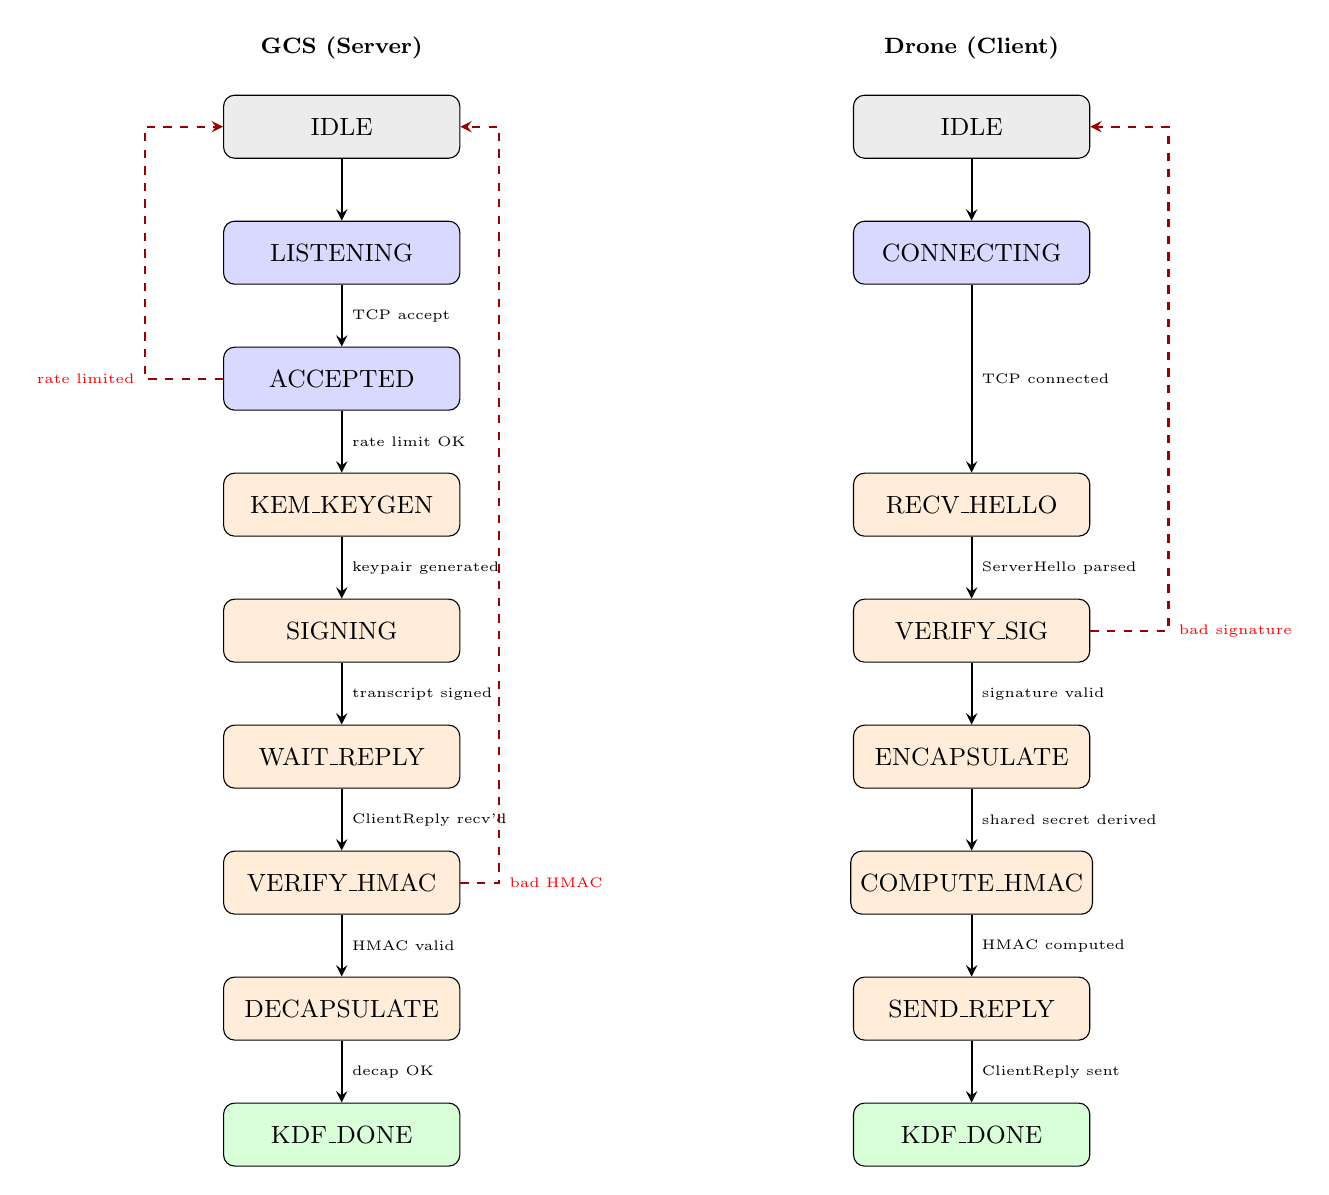
\begin{tikzpicture}[
    state/.style={draw, rounded corners, minimum width=3cm, minimum height=0.8cm,
                  font=\small, align=center},
    trans/.style={->, thick, >=stealth},
    fail/.style={->, thick, >=stealth, red!60!black, dashed},
    node distance=1.6cm,
  ]
    % GCS states
    \node[font=\footnotesize\bfseries] at (-4, 1) {GCS (Server)};
    \node[state, fill=gray!15]   (gi) at (-4, 0)   {IDLE};
    \node[state, fill=blue!15]   (gl) at (-4, -1.6) {LISTENING};
    \node[state, fill=blue!15]   (ga) at (-4, -3.2) {ACCEPTED};
    \node[state, fill=orange!15] (gk) at (-4, -4.8) {KEM\_KEYGEN};
    \node[state, fill=orange!15] (gs) at (-4, -6.4) {SIGNING};
    \node[state, fill=orange!15] (gw) at (-4, -8.0) {WAIT\_REPLY};
    \node[state, fill=orange!15] (gv) at (-4, -9.6) {VERIFY\_HMAC};
    \node[state, fill=orange!15] (gd) at (-4, -11.2) {DECAPSULATE};
    \node[state, fill=green!15]  (gf) at (-4, -12.8) {KDF\_DONE};

    \draw[trans] (gi) -- (gl);
    \draw[trans] (gl) -- node[right, font=\tiny] {TCP accept} (ga);
    \draw[trans] (ga) -- node[right, font=\tiny] {rate limit OK} (gk);
    \draw[trans] (gk) -- node[right, font=\tiny] {keypair generated} (gs);
    \draw[trans] (gs) -- node[right, font=\tiny] {transcript signed} (gw);
    \draw[trans] (gw) -- node[right, font=\tiny] {ClientReply recv'd} (gv);
    \draw[trans] (gv) -- node[right, font=\tiny] {HMAC valid} (gd);
    \draw[trans] (gd) -- node[right, font=\tiny] {decap OK} (gf);
    \draw[fail]  (ga) -- ++(-2.5,0) node[left, font=\tiny, red] {rate limited} |- (gi);
    \draw[fail]  (gv) -- ++(2,0) node[right, font=\tiny, red] {bad HMAC} |- (gi);

    % Drone states
    \node[font=\footnotesize\bfseries] at (4, 1) {Drone (Client)};
    \node[state, fill=gray!15]   (di) at (4, 0)   {IDLE};
    \node[state, fill=blue!15]   (dc) at (4, -1.6) {CONNECTING};
    \node[state, fill=orange!15] (dr) at (4, -4.8) {RECV\_HELLO};
    \node[state, fill=orange!15] (dv) at (4, -6.4) {VERIFY\_SIG};
    \node[state, fill=orange!15] (de) at (4, -8.0) {ENCAPSULATE};
    \node[state, fill=orange!15] (dh) at (4, -9.6) {COMPUTE\_HMAC};
    \node[state, fill=orange!15] (ds) at (4, -11.2) {SEND\_REPLY};
    \node[state, fill=green!15]  (df) at (4, -12.8) {KDF\_DONE};

    \draw[trans] (di) -- (dc);
    \draw[trans] (dc) -- node[right, font=\tiny] {TCP connected} (dr);
    \draw[trans] (dr) -- node[right, font=\tiny] {ServerHello parsed} (dv);
    \draw[trans] (dv) -- node[right, font=\tiny] {signature valid} (de);
    \draw[trans] (de) -- node[right, font=\tiny] {shared secret derived} (dh);
    \draw[trans] (dh) -- node[right, font=\tiny] {HMAC computed} (ds);
    \draw[trans] (ds) -- node[right, font=\tiny] {ClientReply sent} (df);
    \draw[fail]  (dv) -- ++(2.5,0) node[right, font=\tiny, red] {bad signature} |- (di);
  \end{tikzpicture}
  \caption{Handshake state machines for GCS (server) and drone (client).
           Green = terminal success.  Red dashed = failure paths.}
  \label{fig:ps-handshake-fsm}
\end{figure}

\paragraph{State Transitions.}

\begin{longtable}{l l l p{5cm}}
  \caption{GCS handshake state transitions.}
  \label{tab:ps-gcs-transitions} \\
  \toprule
  \textbf{From} & \textbf{To} & \textbf{Trigger} & \textbf{Action} \\
  \midrule
  \endfirsthead
  \bottomrule
  \endfoot

  IDLE       & LISTENING    & Start signal      & Bind TCP socket to port 46000 \\
  LISTENING  & ACCEPTED     & TCP SYN received  & \texttt{accept()}, record peer IP \\
  ACCEPTED   & KEM\_KEYGEN  & Rate limit passes & Call \texttt{KEM.keygen()} \\
  ACCEPTED   & IDLE         & Rate limit fails  & Close TCP, log attempt \\
  KEM\_KEYGEN & SIGNING     & Keypair ready     & Build transcript, call \texttt{SIG.sign()} \\
  SIGNING    & WAIT\_REPLY  & Signature ready   & Serialize \& send ServerHello \\
  WAIT\_REPLY & VERIFY\_HMAC & Data received    & Parse ClientReply \\
  VERIFY\_HMAC & DECAPSULATE & HMAC matches    & Call \texttt{KEM.decap()} \\
  VERIFY\_HMAC & IDLE        & HMAC mismatch    & Log, close TCP \\
  DECAPSULATE & KDF\_DONE   & Shared secret OK  & HKDF $\to$ key\_d2g, key\_g2d \\
\end{longtable}

% ────────────────────────────────────────────────────────────────────────────
\section{Data Plane State Machine}
\label{sec:ps-data-fsm}

After the handshake succeeds, the proxy enters the data-plane
event loop.  The data plane has three states:

\begin{figure}[H]
  \centering
  \begin{tikzpicture}[
    state/.style={draw, rounded corners, minimum width=3.5cm, minimum height=1cm,
                  font=\small, align=center, fill=#1},
    trans/.style={->, thick, >=stealth},
    node distance=2.5cm,
  ]
    \node[state=green!15]  (active) {ACTIVE\\(encrypting/decrypting)};
    \node[state=yellow!15, below left=of active] (blackout) {BLACKOUT\\(rekey in progress)};
    \node[state=red!15, below right=of active]  (stopped) {STOPPED\\(terminated)};

    \draw[trans] (active)   -- node[left, font=\tiny, align=right] {rekey\\triggered} (blackout);
    \draw[trans] (blackout) -- node[below, font=\tiny] {handshake OK} (active);
    \draw[trans] (blackout) -- node[right, font=\tiny, align=left] {handshake\\failed} (stopped);
    \draw[trans] (active)   -- node[right, font=\tiny, align=left] {stop\\signal} (stopped);
  \end{tikzpicture}
  \caption{Data-plane state machine.}
  \label{fig:ps-data-fsm}
\end{figure}

\begin{description}
  \item[ACTIVE:]
    The steady-state.  The proxy encrypts plaintext packets and decrypts
    encrypted packets.  The sequence number increments monotonically.

  \item[BLACKOUT:]
    Entered when a rekey is triggered (by the policy engine or scheduler).
    During blackout, no new packets are encrypted.  Incoming encrypted
    packets may still be processed if they belong to the current session.
    A new TCP handshake is performed.  If the handshake succeeds, the
    proxy transitions back to ACTIVE with new keys.

  \item[STOPPED:]
    Terminal state.  Reached on normal shutdown or unrecoverable error.
    All sockets are closed and key material is released.
\end{description}

% ────────────────────────────────────────────────────────────────────────────
\section{Replay Window Specification}
\label{sec:ps-replay}

The anti-replay mechanism is specified by three parameters:

\begin{table}[H]
  \centering
  \caption{Replay window parameters.}
  \label{tab:ps-replay-params}
  \begin{tabular}{l l l}
    \toprule
    \textbf{Parameter} & \textbf{Default} & \textbf{Description} \\
    \midrule
    \texttt{window}  & 1024 & Maximum out-of-order tolerance (packets). \\
    \texttt{\_high}  & $-1$ & Highest sequence number accepted so far. \\
    \texttt{\_mask}  & 0    & Bitmask of received sequence numbers within window. \\
    \bottomrule
  \end{tabular}
\end{table}

\paragraph{Accept/Reject Algorithm.}
Given an incoming sequence number $s$:

\begin{lstlisting}[style=python, caption={Anti-replay window algorithm}]
def check(self, seq: int) -> bool:
    if seq > self._high:
        # New packet ahead of window: shift and accept
        shift = seq - self._high
        self._mask = (self._mask << shift) | 1
        self._high = seq
        return True
    
    offset = self._high - seq
    if offset >= self.window:
        return False   # Too old: reject
    
    bit = 1 << offset
    if self._mask & bit:
        return False   # Already seen: reject (replay)
    
    self._mask |= bit  # Mark as seen: accept
    return True
\end{lstlisting}

\paragraph{Window Size Justification.}
A window of 1024~packets tolerates significant UDP reordering.
At 50~packets/second (typical MAVLink telemetry rate), the window
covers 20.5~seconds of traffic---sufficient for any realistic WiFi
reordering scenario.

% ────────────────────────────────────────────────────────────────────────────
\section{Scheduler Control Protocol}
\label{sec:ps-scheduler}

The benchmark scheduler uses a JSON-over-TCP protocol on port~48080.
Each message is a newline-delimited JSON object (\texttt{\textbackslash n}-terminated).

\subsection{Message Types}

\begin{longtable}{l l p{6cm}}
  \caption{Scheduler control protocol message types.}
  \label{tab:ps-scheduler-msgs} \\
  \toprule
  \textbf{Type} & \textbf{Direction} & \textbf{Description} \\
  \midrule
  \endfirsthead
  \bottomrule
  \endfoot

  \texttt{start\_proxy} & Drone $\to$ GCS & Start GCS proxy with specified suite.
    Fields: \texttt{suite\_id}, \texttt{mode}, \texttt{sig\_pub\_path}. \\
  \texttt{stop\_proxy}  & Drone $\to$ GCS & Stop the current GCS proxy process. \\
  \texttt{start\_mav}   & Drone $\to$ GCS & Start GCS MAVProxy with specified ports. \\
  \texttt{stop\_mav}    & Drone $\to$ GCS & Stop the current GCS MAVProxy process. \\
  \texttt{status}        & Drone $\to$ GCS & Request GCS status (proxy running, MAV running). \\
  \texttt{clock\_sync}   & Drone $\to$ GCS & Chronos clock synchronisation exchange. \\
  \texttt{ack}           & GCS $\to$ Drone & Acknowledge a command.  Fields: \texttt{ok}, \texttt{error}. \\
  \texttt{status\_reply} & GCS $\to$ Drone & Response to status query. \\
\end{longtable}

\paragraph{Example Exchange.}

\begin{lstlisting}[style=terminal, caption={Scheduler protocol exchange (JSON over TCP)}]
# Drone sends:
{"type":"start_proxy","suite_id":"cs-mlkem768-aesgcm-mldsa65",
 "mode":"gcs","sig_pub_path":"keys/gcs_mldsa65.pub"}\n

# GCS responds:
{"type":"ack","ok":true}\n

# Drone sends:
{"type":"start_mav","udp_in":47001,"udp_out":47002}\n

# GCS responds:
{"type":"ack","ok":true}\n

# ... benchmark runs for 110 seconds ...

# Drone sends:
{"type":"stop_mav"}\n
{"type":"stop_proxy"}\n
\end{lstlisting}

\begin{securitynote}
The scheduler control protocol is \textbf{unauthenticated and unencrypted}.
Any host on the LAN can inject commands.  This is acceptable for a
controlled lab benchmark but must be secured (TLS or HMAC) for any
production deployment.
\end{securitynote}

% ────────────────────────────────────────────────────────────────────────────
\section{Policy Engine Protocol}
\label{sec:ps-policy}

The suite scheduling policy follows a two-phase commit protocol:

\subsection{Phase 1: Evaluate (Read-Only)}

\begin{lstlisting}[style=python, caption={Policy evaluate interface}]
@dataclass
class PolicyDecision:
    action: str          # "STAY" | "NEXT_SUITE" | "FINISH"
    reason: str          # Human-readable explanation
    remaining_s: float   # Seconds remaining in current suite

decision = policy.evaluate(
    elapsed_s=elapsed,
    metrics=current_metrics,
    suite_index=current_index,
    total_suites=total
)
\end{lstlisting}

\texttt{evaluate()} is a \textbf{pure function}: it reads state but
does not modify it.  Multiple calls with the same inputs produce the
same output.

\subsection{Phase 2: Confirm (State Mutation)}

\begin{lstlisting}[style=python, caption={Policy confirm interface}]
new_index = policy.confirm_advance(
    current_index=current_index,
    total_suites=total
)
\end{lstlisting}

\texttt{confirm\_advance()} increments the suite index.  It is called
\textbf{only after} the scheduler has:
\begin{enumerate}
  \item Stopped the current proxy and MAVProxy processes.
  \item Written the current suite's metrics to the JSONL output.
  \item Verified the file write succeeded.
\end{enumerate}

This separation prevents the ``metrics attributed to wrong suite'' bug.

% ────────────────────────────────────────────────────────────────────────────
\section{Metrics Output Format}
\label{sec:ps-metrics}

Benchmark metrics are written to a JSONL file (one JSON object per line).
Each line represents one suite's benchmark results.

\paragraph{Top-Level Structure.}

\begin{lstlisting}[style=python, caption={Metrics JSONL record structure}]
{
  "suite_id": "cs-mlkem768-aesgcm-mldsa65",
  "suite_index": 0,
  "timestamp_utc": "2024-12-15T14:30:00.123456Z",
  "elapsed_s": 110.0,
  "categories": {
    "A": { ... },   // Environment
    "B": { ... },   // Handshake timing
    "C": { ... },   // Data-plane counters
    // ... through "R"
  }
}
\end{lstlisting}

The 18~metric categories (A through R) are documented in
Chapter~\ref{ch:metrics} and Appendix~\ref{app:schema}.

% ────────────────────────────────────────────────────────────────────────────
\section{Error Code Registry}
\label{sec:ps-errors}

The system defines a hierarchy of custom exceptions:

\begin{longtable}{l l p{5cm}}
  \caption{Exception hierarchy.}
  \label{tab:ps-errors} \\
  \toprule
  \textbf{Exception} & \textbf{Parent} & \textbf{Meaning} \\
  \midrule
  \endfirsthead
  \bottomrule
  \endfoot

  \texttt{SecureTunnelError}    & \texttt{Exception}            & Base for all system errors. \\
  \texttt{HandshakeError}       & \texttt{SecureTunnelError}    & General handshake failure. \\
  \texttt{HandshakeFormatError} & \texttt{HandshakeError}       & Malformed wire message. \\
  \texttt{HandshakeVerifyError} & \texttt{HandshakeError}       & Crypto verification failed. \\
  \texttt{AeadError}            & \texttt{SecureTunnelError}    & AEAD framing error. \\
  \texttt{SequenceOverflow}     & \texttt{AeadError}            & Sequence number exhausted. \\
  \texttt{HeaderMismatch}       & \texttt{AeadError}            & Header field mismatch. \\
  \texttt{ReplayError}          & \texttt{AeadError}            & Anti-replay check failed. \\
  \texttt{AeadAuthError}        & \texttt{AeadError}            & AEAD tag verification failed. \\
  \texttt{PolicyError}          & \texttt{SecureTunnelError}    & Policy evaluation failure. \\
  \texttt{ProcessError}         & \texttt{SecureTunnelError}    & Managed subprocess failure. \\
  \texttt{CollectorError}       & \texttt{SecureTunnelError}    & Metrics collector failure. \\
\end{longtable}

% ────────────────────────────────────────────────────────────────────────────
\section{Configuration Key Specification}
\label{sec:ps-config}

All runtime configuration is centralised in the \texttt{CONFIG} dictionary
in \filename{core/config.py}.  Environment variables override defaults
using the naming convention \texttt{SECDRONE\_<KEY>}.

\begin{longtable}{l l l p{4cm}}
  \caption{Configuration keys (security-critical subset).}
  \label{tab:ps-config-security} \\
  \toprule
  \textbf{Key} & \textbf{Type} & \textbf{Default} & \textbf{Security Impact} \\
  \midrule
  \endfirsthead
  \toprule
  \textbf{Key} & \textbf{Type} & \textbf{Default} & \textbf{Security Impact} \\
  \midrule
  \endhead
  \bottomrule
  \endfoot

  \texttt{DRONE\_PSK}             & str (base64) & (none)   & Pre-shared key for drone auth.  Must be $\geq$32 bytes decoded. \\
  \texttt{GCS\_SIG\_PRIVATE\_KEY} & path         & (none)   & GCS signing private key file.  Must be restricted to owner. \\
  \texttt{GCS\_SIG\_PUBLIC\_KEY}  & path         & (none)   & GCS signing public key.  Pre-installed on drone. \\
  \texttt{STRICT\_UDP\_PEER\_MATCH} & bool       & True     & Reject encrypted packets from unexpected IPs. \\
  \texttt{REPLAY\_WINDOW}         & int          & 1024     & Anti-replay window size.  Smaller = more secure, less tolerant. \\
  \texttt{REKEY\_SEQ\_THRESHOLD}  & int          & $2^{63}$ & Force rekey before this sequence number. \\
  \texttt{RATE\_LIMIT\_CAPACITY}  & int          & 5        & Token bucket capacity for handshake rate limiting. \\
  \texttt{RATE\_LIMIT\_REFILL}    & float        & 3.0      & Tokens per second for rate limiting. \\
  \texttt{UDP\_DSCP\_VALUE}       & int          & 0        & DSCP marking for QoS prioritisation. \\
  \texttt{HANDSHAKE\_TIMEOUT}     & float        & 60.0     & TCP handshake timeout (seconds). \\
\end{longtable}

% ────────────────────────────────────────────────────────────────────────────
\section{Summary}
\label{sec:ps-summary}

This chapter provided a byte-level specification of:

\begin{itemize}
  \item \textbf{Three wire message types}: ServerHello (TCP), ClientReply (TCP),
        and EncryptedDatagram (UDP).
  \item \textbf{Algorithm identifier registries}: Numeric IDs for 9 KEMs and
        8 signatures, embedded in every data-plane packet header.
  \item \textbf{Key derivation}: HKDF-SHA256 with domain-separated salt and
        info, producing two 32-byte directional transport keys.
  \item \textbf{Handshake state machine}: 9 states for GCS, 8 states for drone,
        with explicit failure paths.
  \item \textbf{Data plane state machine}: ACTIVE, BLACKOUT, and STOPPED states
        with rekey transitions.
  \item \textbf{Replay window}: Bitmask-based sliding window with configurable
        size (default 1024 packets).
  \item \textbf{Scheduler control protocol}: JSON-over-TCP commands for
        benchmark orchestration.
  \item \textbf{Policy engine protocol}: Two-phase commit (evaluate + confirm)
        for suite rotation.
  \item \textbf{Error hierarchy}: 11 custom exceptions with specific meanings.
  \item \textbf{Configuration keys}: Security-critical subset with defaults
        and override mechanisms.
\end{itemize}

This specification is sufficient for an independent implementer to create
an interoperable client or server without reading the Python source code.
